\newcommand{\verilogfolderGateAND}{./componentes}
\newcommand{\imagesfolderGateAND}{./componentes}

%#######################################################################
%#######################################################################
%% Compuerta lógica: AND (1)
%#######################################################################
%#######################################################################
\section{Compuerta lógica: AND (1)}\index{Compuerta lógica: AND (1)}
\normalsize
A continuación se presenta el componente combinacional \textbf{Compuerta Lógica AND} mostrando su descripción con ecuación lógica.
%#######################################################################
%#######################################################################
%% Descripción del componente
%#######################################################################
%#######################################################################
\subsection{Descripción del componente}\index{Descripción del componente}
\scriptsize
	\begin{tcolorbox}[enhanced,title=PRODUCTO DE CALIDAD:,colframe=colorA1,colback=colorA2,arc=0mm,colbacktitle=white,fonttitle=\bfseries,coltitle=white,attach boxed title to top left={xshift=3.2mm,yshift=-0.50mm},boxed title style={skin=enhancedfirst jigsaw,size=small,arc=0mm,bottom=1mm,interior style={fill=none,top color=color2,bottom color=color2},,boxrule=0pt},boxrule=0pt]
	OBJETIVO PEDAGÓGICO: El estudiante identifica las especificaciones y restricciones (enunciadas y no enunciadas del componente) para comprender el requerimiento solicitado. \\
	ENTREGABLES: Contiene máximo dos párrafos (claros, precisos y coherentes) que explican: restricciones, especificaciones y búsqueda e identificación de contextos en donde se utiliza dicho componente.
		\begin{enumerate}
			\item[a.] La descripción del componente está redactada en palabras propias de los estudiantes, organizada lógica y claramente. 
			\item[b.] Las especificaciones y restricciones responden totalmente al componente solicitado, demostrando originalidad y aportes propios.
			\item[c.] La búsqueda e identificación de características similares de proyectos base utilizados como referencia es clara justificando su utilidad para el desarrollo del proyecto.
			\item[d.] El lenguaje disciplinar es preciso y adecuado, las frases son gramaticalmente correctas y no hay errores ortográficos. 	
		\end{enumerate}
	\end{tcolorbox}

\normalsize

	La compuerta lógica AND es uno de los elementos más simples de la electrónica digital. Una compuerta AND de 2 entradas toma  a la salida un valor de uno (1-lógico, nivel alto) cuando las dos entradas están en valor de uno. Así mismo, las compuertas AND pueden tener más de dos entradas en donde la salida toma un valor de 1-lógico si todas las entradas tiene valor de 1-lógico en cualquier otro caso la salida toma un valor de 0-lógico. \\
	
	Una compuerta AND así como todas las compuertas básicas forman parte de cualquier circuito digital, sin embargo, una compuerta AND no es un componente funcionalmente completo, lo que quiere decir que solo con compuertas AND no se puede construir toda la electrónica digital, porque con la compuerta AND no se pueden implementar las demás compuertas.\\
%#######################################################################
%#######################################################################
%% Símbolo
%#######################################################################
%#######################################################################
\subsection{Símbolo}\index{Símbolo}
\scriptsize
		\begin{tcolorbox}[enhanced,title=PRODUCTO DE CALIDAD:,colframe=colorA1,colback=colorA2,arc=0mm,colbacktitle=white,fonttitle=\bfseries,coltitle=white,attach boxed title to top left={xshift=3.2mm,yshift=-0.50mm},boxed title style={skin=enhancedfirst jigsaw,size=small,arc=0mm,bottom=1mm,interior style={fill=none,top color=color2,bottom color=color2},,boxrule=0pt},boxrule=0pt]
		OBJETIVO PEDAGÓGICO: El estudiante es capaz de relacionar el componente a diseñar con un símbolo genérico para poder usarlo en un diagrama arquitectural.\\
		ENTREGABLES: Diagrama correcto y completo.
		\begin{enumerate}
			\item[a.] El símbolo propuesto para representar el componente se basa en símbolos de naturaleza similar presentados en la literatura de componentes electrónicos.
		\end{enumerate}
	\end{tcolorbox}

\normalsize

		\begin{center}
			
\includegraphics[width=0.8\linewidth]{\imagesfolderGateAND/GateAND/SYM_GateAND.pdf}%
		\end{center}
%#######################################################################
%#######################################################################
%% Diagrama caja negra
%#######################################################################
%#######################################################################
\subsection{Diagrama caja negra}\index{Diagrama caja negra}
\scriptsize
		\begin{tcolorbox}[enhanced,title=PRODUCTO DE CALIDAD:,colframe=colorA1,colback=colorA2,arc=0mm,colbacktitle=white,fonttitle=\bfseries,coltitle=white,attach boxed title to top left={xshift=3.2mm,yshift=-0.50mm},boxed title style={skin=enhancedfirst jigsaw,size=small,arc=0mm,bottom=1mm,interior style={fill=none,top color=color2,bottom color=color2},,boxrule=0pt},boxrule=0pt]
		OBJETIVO PEDAGÓGICO: El estudiante es capaz de realizar un diagrama de caja negra para identificar señales de entrada/salida del producto.\\
		ENTREGABLES: Diagrama correcto y completo.
		\begin{enumerate}
			\item[a.] El diagrama de caja negra muestra todas las señales de entrada y salida con sus correspondientes nombres estructurados (In/Out) y tamaños (bit/bus).
			\item[b.] El diagrama de caja negra relaciona dicho componente con el diagrama de caracterización (test-bench).
		\end{enumerate}
	\end{tcolorbox}

\normalsize

%\begin{landscape}

		\begin{center}
			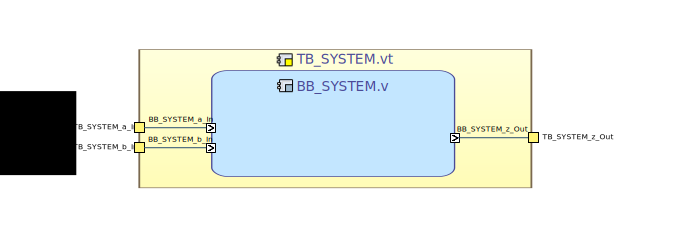
\includegraphics[width=1\linewidth]{\imagesfolderGateAND/GateAND/BB_GateAND.jpg}%
		\end{center}
%#######################################################################
%#######################################################################
%% Funcionalidad: ecuación característica y/o tabla de verdad y/o macro algoritmo general
%#######################################################################
%#######################################################################
\subsection{Funcionalidad}\index{Funcionalidad}
\scriptsize
	\begin{tcolorbox}[enhanced,title=PRODUCTO DE CALIDAD:,colframe=colorA1,colback=colorA2,arc=0mm,colbacktitle=white,fonttitle=\bfseries,coltitle=white,attach boxed title to top left={xshift=3.2mm,yshift=-0.50mm},boxed title style={skin=enhancedfirst jigsaw,size=small,arc=0mm,bottom=1mm,interior style={fill=none,top color=color2,bottom color=color2},,boxrule=0pt},boxrule=0pt]
		OBJETIVO PEDAGÓGICO: El estudiante es capaz de proponer macroalgoritmos descomponiendo el problema en un conjunto de pasos para detallar la funcionalidad esperada del componente. \\
		ENTREGABLES: Ecuación / Tabla de Verdad / Macro-algoritmo correcto y completo según funcionalidad del componente.
		\begin{enumerate}
			\item[a.] El macro-algoritmo de solución describe correctamente la funcionalidad del producto y se representa adecuadamente con una explicación detallada en donde cada paso es menos complejo que el producto solicitado. 
			\item[b.] En cada paso del macro-algoritmo se detalla correctamente un pseudo-algoritmo que describe una posible implementación.
		\end{enumerate}
	\end{tcolorbox}

\normalsize
	%-----------------------------------------------------------------------
		\begin{remark}
			\textbf{Ecuación característica}
		\end{remark}
		\begin{center}	
			\textit{CC\_GateAND\_z\_Out} \textcolor{red}{<=} \textit{CC\_GateAND\_a\_In} \textcolor{red}{and} \textit{CC\_GateAND\_a\_In}; \\
		\end{center}
	%-----------------------------------------------------------------------
		\begin{remark}
			\textbf{Tabla de verdad}
		\end{remark}
		\begin{center}	
			\begin{tabular}{|c|c|c|}
			\hline
			\multicolumn{2}{|c|}{\cellcolor{colorIN1}\textbf{INPUTS}} & \multicolumn{1}{c|}{\cellcolor{colorOUT1}\textbf{OUTPUTS}} \\ \hline
			\cellcolor{colorIN1}\textbf{CC\_GateAND\_a\_In} 	& \cellcolor{colorIN1}\textbf{CC\_GateAND\_b\_In} 	& 	\cellcolor{colorOUT1} \textbf{CC\_GateAND\_z\_Out}	\\ \hline
			\cellcolor{colorIN2} 0								& \cellcolor{colorIN2} 0							& 	\cellcolor{colorOUT2} 0								\\ \hline
			\cellcolor{colorIN2} 0								& \cellcolor{colorIN2} 1							& 	\cellcolor{colorOUT2} 0								\\ \hline
			\cellcolor{colorIN2} 1								& \cellcolor{colorIN2} 0							& 	\cellcolor{colorOUT2} 0								\\ \hline
			\cellcolor{colorIN2} 1								& \cellcolor{colorIN2} 1							& 	\cellcolor{colorOUT2} 1								\\ \hline
			\end{tabular}
		\end{center}
	%-----------------------------------------------------------------------
		\begin{remark}
			\textbf{Macro algoritmo}
		\end{remark}
			\begin{algorithm}[H]
			\SetAlgoLined
				\KwData{$CC\_GateAND\_a\_In$, $CC\_GateAND\_b\_In$ ~(0, 1)}
				\KwResult{$CC\_GateAND\_z\_Out$ ~(0, 1)}
			%initialization\;
					$CC\_GateAND\_z\_Out$ \textcolor{red}{=} $CC\_GateAND\_a\_In$ \textcolor{red}{and} $CC\_GateAND\_b\_In$
				\caption{Compuerta lógica AND}
			\end{algorithm}

		\begin{center}
			\includegraphics[width=0.5\linewidth]{\imagesfolderGateAND/GateAND/FC_GateAND_1.jpg}%
		\end{center}
	%-----------------------------------------------------------------------
%#######################################################################
%#######################################################################
%% HDL: Caja negra
%#######################################################################
%#######################################################################
\subsection{HDL: Caja negra}\index{HDL: Caja negra}
\scriptsize
	\begin{tcolorbox}[enhanced,title=PRODUCTO DE CALIDAD:,colframe=colorA1,colback=colorA2,arc=0mm,colbacktitle=white,fonttitle=\bfseries,coltitle=white,attach boxed title to top left={xshift=3.2mm,yshift=-0.50mm},boxed title style={skin=enhancedfirst jigsaw,size=small,arc=0mm,bottom=1mm,interior style={fill=none,top color=color2,bottom color=color2},,boxrule=0pt},boxrule=0pt]
		OBJETIVO PEDAGÓGICO: El estudiante es capaz de describir lo solicitado en lenguajes de HDL para identificar los elementos básicos de la herramienta de diseño y del lenguaje. \\
		ENTREGABLES: Códigos fuente.
		\begin{enumerate}
			\item[a.] La descripción en lenguajes hardware (complejidad del código, diferencia combinacional y secuencial) es correcta y corresponde al producto solicitado.
			\item[b.] Se incluye documentación completa para estructurar y/o entender el código claramente (indentación y sintaxis de los lenguajes), nombrando correcta y adecuadamente todas las señales, variables y demás elementos relevantes. 
		\end{enumerate}
	\end{tcolorbox}

\normalsize

	%-----------------------------------------------------------------------
	\lstinputlisting[language=Verilog,caption=BB\_SYSTEM.v]{\verilogfolderGateAND/PRJ0_GateAND_1/BB_SYSTEM.v1BB}
	%-----------------------------------------------------------------------
%#######################################################################
%#######################################################################
%% Definición vectores de prueba
%#######################################################################
%#######################################################################
\subsection{Definición vectores de prueba}\index{Definición vectores de prueba}
\scriptsize
	\begin{tcolorbox}[enhanced,title=PRODUCTO DE CALIDAD:,colframe=colorA1,colback=colorA2,arc=0mm,colbacktitle=white,fonttitle=\bfseries,coltitle=white,attach boxed title to top left={xshift=3.2mm,yshift=-0.50mm},boxed title style={skin=enhancedfirst jigsaw,size=small,arc=0mm,bottom=1mm,interior style={fill=none,top color=color2,bottom color=color2},,boxrule=0pt},boxrule=0pt]
		OBJETIVO PEDAGÓGICO: El estudiante es capaz de proponer una estrategia de identificación de vectores de prueba para validar la funcionalidad del componente.\\
		ENTREGABLES: Estrategias claras de selección. Explicación clara de funcionamiento.
		\begin{enumerate}
			\item[a.] Los vectores de prueba se seleccionan a partir de una estrategia explícita y claramente definida expresada en un párrafo. Estos vectores permiten comprobar totalmente la funcionalidad del componente. Se realizan simulaciones funcionales que validan esos vectores de prueba. 
		\end{enumerate}
	\end{tcolorbox}

\normalsize

	En este caso como son pocas entradas se debe validar toda la tabla de verdad. Los vectores de prueba corresponden entonces a dichas combinaciones así:
		\begin{center}
			\begin{tabular}{|c|c|c|}
			\hline
			\multicolumn{2}{|c|}{\cellcolor{colorIN1}\textbf{INPUTS}} & \multicolumn{1}{c|}{\cellcolor{colorOUT1}\textbf{OUTPUTS}} \\ \hline
			\cellcolor{colorIN1}\textbf{CC\_GateAND\_a\_In} 	& \cellcolor{colorIN1}\textbf{CC\_GateAND\_b\_In} 	& 	\cellcolor{colorOUT1} \textbf{CC\_GateAND\_z\_Out}	\\ \hline
			\cellcolor{colorIN2} 0								& \cellcolor{colorIN2} 0							& 	\cellcolor{colorOUT2} ?								\\ \hline
			\cellcolor{colorIN2} 0								& \cellcolor{colorIN2} 1							& 	\cellcolor{colorOUT2} ?								\\ \hline
			\cellcolor{colorIN2} 1								& \cellcolor{colorIN2} 0							& 	\cellcolor{colorOUT2} ?								\\ \hline
			\cellcolor{colorIN2} 1								& \cellcolor{colorIN2} 1							& 	\cellcolor{colorOUT2} ?								\\ \hline
			\end{tabular}
		\end{center}

%#######################################################################
%#######################################################################
%% HDL: Vectores de prueba
%#######################################################################
%#######################################################################
\subsection{HDL: Vectores de prueba}\index{HDL: Vectores de prueba}
\scriptsize
	\begin{tcolorbox}[enhanced,title=PRODUCTO DE CALIDAD:,colframe=colorA1,colback=colorA2,arc=0mm,colbacktitle=white,fonttitle=\bfseries,coltitle=white,attach boxed title to top left={xshift=3.2mm,yshift=-0.50mm},boxed title style={skin=enhancedfirst jigsaw,size=small,arc=0mm,bottom=1mm,interior style={fill=none,top color=color2,bottom color=color2},,boxrule=0pt},boxrule=0pt]
		OBJETIVO PEDAGÓGICO: El estudiante es capaz de describir lo solicitado en lenguajes de HDL para identificar los elementos básicos de la herramienta de diseño y del lenguaje. \\
		ENTREGABLES: Códigos fuente.
		\begin{enumerate}
			\item[a.] La descripción en lenguajes hardware (complejidad del código, diferencia combinacional y secuencial) es correcta y corresponde al producto solicitado.
			\item[b.] Se incluye documentación completa para estructurar y/o entender el código claramente (indentación y sintaxis de los lenguajes), nombrando correcta y adecuadamente todas las señales, variables y demás elementos relevantes. 
		\end{enumerate}
	\end{tcolorbox}

\normalsize

	%-----------------------------------------------------------------------
	\lstinputlisting[language=Verilog,caption=TB\_SYSTEM.vt]{\verilogfolderGateAND/PRJ0_GateAND_1/simulation/modelsim/TB_SYSTEM.vt1}
	%-----------------------------------------------------------------------
%#######################################################################
%#######################################################################
%% Diagrama caja blanca
%#######################################################################
%#######################################################################
\subsection{Diagrama caja blanca}\index{Diagrama caja blanca}
\scriptsize
	\begin{tcolorbox}[enhanced,title=PRODUCTO DE CALIDAD:,colframe=colorA1,colback=colorA2,arc=0mm,colbacktitle=white,fonttitle=\bfseries,coltitle=white,attach boxed title to top left={xshift=3.2mm,yshift=-0.50mm},boxed title style={skin=enhancedfirst jigsaw,size=small,arc=0mm,bottom=1mm,interior style={fill=none,top color=color2,bottom color=color2},,boxrule=0pt},boxrule=0pt]
		OBJETIVO PEDAGÓGICO: El estudiante es capaz de realizar un diagrama con sub-componentes, señales e interconexiones para mostrar un diseño estructurado que permita llegar a una implementación del componente.\\
		ENTREGABLES: Diagrama de sub-componentes, señales e interconexiones, descripción de componente o componente a componente.
		\begin{enumerate}
			\item[a.] El diagrama de caja blanca es correcto y corresponde con el componente solicitado. 
			\item[b.] Se muestran todas las señales de entrada/salida e internas con sus correspondientes nombres estructurados (In/Out) y tamaños (Bit/Bus) para todos los componentes internos del sistema.
			\item[c.] El diagrama de caja blanca corresponde a una solución eficiente en cuanto a recursos, número de bloques y elementos y algoritmo de solución. Los componentes internos son menos complejos que los de mayor jerarquía.
			\item[d.] Se presenta una descripción (qué es y cómo funciona) de cada uno de los componentes constitutivos del componente solicitado, describiendo sus señales.
		\end{enumerate}
	\end{tcolorbox}

\normalsize

		En este caso el diagrama corresponde solamente a la compuerta.
		\begin{center}
			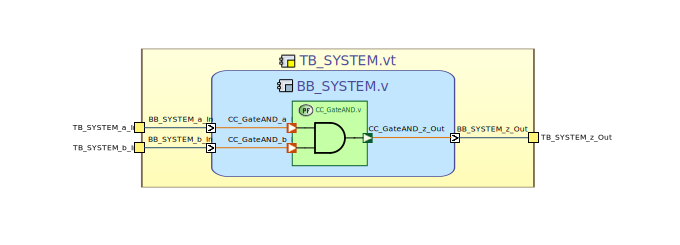
\includegraphics[width=1\linewidth]{\imagesfolderGateAND/GateAND/WB_GateAND.jpg}
		\end{center}
%#######################################################################
%#######################################################################
%% HDL: Caja blanca
%#######################################################################
%#######################################################################
\subsection{HDL: Caja blanca}\index{HDL: Caja blanca}
\scriptsize
	\begin{tcolorbox}[enhanced,title=PRODUCTO DE CALIDAD:,colframe=colorA1,colback=colorA2,arc=0mm,colbacktitle=white,fonttitle=\bfseries,coltitle=white,attach boxed title to top left={xshift=3.2mm,yshift=-0.50mm},boxed title style={skin=enhancedfirst jigsaw,size=small,arc=0mm,bottom=1mm,interior style={fill=none,top color=color2,bottom color=color2},,boxrule=0pt},boxrule=0pt]
		OBJETIVO PEDAGÓGICO: El estudiante es capaz de describir lo solicitado en lenguajes de HDL para identificar los elementos básicos de la herramienta de diseño y del lenguaje. \\
		ENTREGABLES: Códigos fuente.
		\begin{enumerate}
			\item[a.] La descripción en lenguajes hardware (complejidad del código, diferencia combinacional y secuencial) es correcta y corresponde al producto solicitado.
			\item[b.] Se incluye documentación completa para estructurar y/o entender el código claramente (indentación y sintaxis de los lenguajes), nombrando correcta y adecuadamente todas las señales, variables y demás elementos relevantes.  
		\end{enumerate}
	\end{tcolorbox}

\normalsize

	%-----------------------------------------------------------------------
	\lstinputlisting[language=Verilog,caption=BB\_SYSTEM.v]{\verilogfolderGateAND/PRJ0_GateAND_1/BB_SYSTEM.v1WB}
	%-----------------------------------------------------------------------
%#######################################################################
%#######################################################################
%% HDL: bloques
%#######################################################################
%#######################################################################
\subsection{HDL: bloques}\index{HDL: bloques}
\scriptsize
	\begin{tcolorbox}[enhanced,title=PRODUCTO DE CALIDAD:,colframe=colorA1,colback=colorA2,arc=0mm,colbacktitle=white,fonttitle=\bfseries,coltitle=white,attach boxed title to top left={xshift=3.2mm,yshift=-0.50mm},boxed title style={skin=enhancedfirst jigsaw,size=small,arc=0mm,bottom=1mm,interior style={fill=none,top color=color2,bottom color=color2},,boxrule=0pt},boxrule=0pt]
		OBJETIVO PEDAGÓGICO: El estudiante es capaz de describir lo solicitado en lenguajes de HDL para identificar los elementos básicos de la herramienta de diseño y del lenguaje. \\
		ENTREGABLES: Códigos fuente.
		\begin{enumerate}
			\item[a.] La descripción en lenguajes hardware (complejidad del código, diferencia combinacional y secuencial) es correcta y corresponde al producto solicitado.
			\item[b.] Se incluye documentación completa para estructurar y/o entender el código claramente (indentación y sintaxis de los lenguajes), nombrando correcta y adecuadamente todas las señales, variables y demás elementos relevantes. 
		\end{enumerate}
	\end{tcolorbox}

\normalsize

	%-----------------------------------------------------------------------
	\lstinputlisting[language=Verilog,caption=CC\_GateAND.v]{\verilogfolderGateAND/PRJ0_GateAND_1/rtl/CC_GateAND.v1}
	%-----------------------------------------------------------------------
%#######################################################################
%#######################################################################
%% Simulación temporal
%#######################################################################
%#######################################################################
\subsection{Simulación temporal}\index{Simulación temporal}
\scriptsize
	\begin{tcolorbox}[enhanced,title=PRODUCTO DE CALIDAD:,colframe=colorA1,colback=colorA2,arc=0mm,colbacktitle=white,fonttitle=\bfseries,coltitle=white,attach boxed title to top left={xshift=3.2mm,yshift=-0.50mm},boxed title style={skin=enhancedfirst jigsaw,size=small,arc=0mm,bottom=1mm,interior style={fill=none,top color=color2,bottom color=color2},,boxrule=0pt},boxrule=0pt]
	OBJETIVO PEDAGÓGICO: El estudiante es capaz de relacionar la funcionalidad según las especificaciones propuestas con diversos tipos de pruebas para comprobar el funcionamiento del componente según lo solicitado. \\
	ENTREGABLES: Diagramas temporales donde se demuestre funcionalidad según las especificaciones propuestas y en diversos tipos de pruebas.
		\begin{enumerate}
			\item[a.] Se presentan resultados de simulación para el producto solicitado, explicando tres o más casos de funcionamiento sobre el diagrama de simulación. La simulación contiene marcadores en la gráfica que señalan situaciones específicas del producto.
		\end{enumerate}
	\end{tcolorbox}

\normalsize

A continuación se presenta un diagrama de lo que se espera obtener del sistema. En este caso que es sencillo se puede hacer un diagrama de tiempos inicial para ver el comportamiento esperado.

		\begin{tikztimingtable}
			\\ % Gives vertical space
			$CC\_GateAND\_a\_In$	& 2L 2H 2L 2H 2L 2H 2L 2H 2L \\ % starts with edge
			$CC\_GateAND\_b\_In$	& 2L 2L 2H 2H 2L 2L 2H 2H 2L \\ % starts with edge
			\\ % Gives vertical space
			$CC\_GateAND\_z\_Out$	&	2L 2L 2L 2H 2L 2L 2L 2H 2L\\
			\extracode
			%~ \begin{scope}[on background layer]
				%~ \vertlines[help lines,opacity=0.3]{}
			%~ \end{scope}
			\begin{pgfonlayer}{background}
				\vertlines[help lines, dotted]{0,2,...,18}
				\foreach \i [count=\col from 0] in {0,2,...,18}
				\node[font=\scriptsize] at (\i,2) {$t_{\col}$};
				\end{pgfonlayer}
		\end{tikztimingtable}

Por otro lado, se presenta el diagrama de tiempos obtenido en la herramienta Quartus de Altera. En este caso podemos ver como coincide con lo esperado. Es muy importante resaltar los casos de simulación, marcando los vectores de prueba en los resultados de simulación.

		\begin{center}
			\includegraphics[width=1\linewidth]{\imagesfolderGateAND/GateAND/ST_GateAND.pdf}%
		\end{center}
%#######################################################################
%#######################################################################
%% Diagramas QUARTUS
%#######################################################################
%#######################################################################
\subsection{Diagramas QUARTUS}\index{Diagramas QUARTUS}
\scriptsize
	\begin{tcolorbox}[enhanced,title=PRODUCTO DE CALIDAD:,colframe=colorA1,colback=colorA2,arc=0mm,colbacktitle=white,fonttitle=\bfseries,coltitle=white,attach boxed title to top left={xshift=3.2mm,yshift=-0.50mm},boxed title style={skin=enhancedfirst jigsaw,size=small,arc=0mm,bottom=1mm,interior style={fill=none,top color=color2,bottom color=color2},,boxrule=0pt},boxrule=0pt]
		OBJETIVO PEDAGÓGICO: El estudiante es capaz de identificar elementos de la Herramienta Quartus para comprender mejor el proceso de diseño.\\
		ENTREGABLES: Diagramas obtenidos en la herramienta.
		\begin{enumerate}
			\item[a.] Se presentan diagramas obtenidos por QUARTUS.
		\end{enumerate}
	\end{tcolorbox}

\normalsize

		\begin{center}
			\includegraphics[width=1\linewidth]{\imagesfolderGateAND/GateAND/Q_GateAND.pdf}%
		\end{center}
%#######################################################################
%#######################################################################
%% Resultados y lecciones aprendidas
%#######################################################################
%#######################################################################
\subsection{Resultados y lecciones aprendidas}\index{Resultados y lecciones aprendidas}
\scriptsize
	\begin{tcolorbox}[enhanced,title=PRODUCTO DE CALIDAD:,colframe=colorA1,colback=colorA2,arc=0mm,colbacktitle=white,fonttitle=\bfseries,coltitle=white,attach boxed title to top left={xshift=3.2mm,yshift=-0.50mm},boxed title style={skin=enhancedfirst jigsaw,size=small,arc=0mm,bottom=1mm,interior style={fill=none,top color=color2,bottom color=color2},,boxrule=0pt},boxrule=0pt]
		OBJETIVO PEDAGÓGICO: El estudiante es capaz de discutir el proceso de diseño para evidenciar problemas, mejoras del componente diseñado.\\
		ENTREGABLES: Contiene máximo dos párrafos (claros, precisos y coherentes).
		\begin{enumerate}
			\item[a.] Se proponen nuevas especificaciones y aplicaciones del trabajo realizado (ejemplo: mayores niveles de complejidad y usos en otros contextos).
			\item[b.] En caso de no lograr el item de funcionamiento glogal; identifica y argumenta las razones principales del no funcionamiento. 
			\item[c.] El lenguaje disciplinar es preciso y adecuado, haciendo uso de frases gramaticalmente correctas, sin errores ortográficos.
		\end{enumerate}
	\end{tcolorbox}

\normalsize

	\begin{tcolorbox}[colback=colorT2,colframe=colorT1,arc=0mm,boxrule=0pt,title=]
		La compuerta lógica AND es uno de los elementos más simples de la electrónica digital y se pude implementar a partir de su ecuación lógica. Además, se pueden realizar una descripción a nivel funcional como se va presentar en la siguiente sección. \\
	\end{tcolorbox}
